\documentclass[aspectratio=169]{beamer}
\usetheme{Malmoe}

\title{Parallel-in-time methods}
\author{Johan Hidding}
\date{2019/03/14}

\begin{document}
    \frame{\titlepage}

    \begin{frame}
        \frametitle{Overview}
        Alternative: skip my talk and read "50 Years of Time Parallel Time Integration" by Martin J. Gander \vspace{20pt}
        \begin{itemize}
            \item Small scale methods
            \item Parareal
            \item MultiGrid
            \item PFASST
        \end{itemize}
    \end{frame}

    \section{Small scale methods}
    \begin{frame}
        \frametitle{ODE Solvers}
        (or PDE through method of lines) \\ \vspace{20pt}
        Initial value problem:
        \[y(t_0) = y_0\]
        \[\dot{y} = f(t, y)\]
    \end{frame}

    \begin{frame}
        \frametitle{(forward) Euler}
        \[y_{i+1} = y_{i} + (t_{i-1} - t_{i}) f(t_{i}, y_{i})\]
        \begin{itemize}
            \item Each $y_i$ depends on $y_{i-1}$.
        \end{itemize}
    \end{frame}

    \begin{frame} 
        \frametitle{Runge-Kutta}
        \[\begin{aligned}
            k_1 &= h\ f(t_i, y_i)\\
            k_2 &= h\ f(t_i + h/2, y_i + k_1/2)\\
            k_3 &= h\ f(t_i + h/2, y_i + k_2/2)\\
            k_4 &= h\ f(t_i + h, y_i + k_3)\\
            y_{i+1} &= y_i + (k_1 + 2k_2 + 2k_3 + k_4)/6
        \end{aligned}\]
        \begin{itemize}
            \item Same problem, even within the method!
        \end{itemize}
    \end{frame}

    \begin{frame}
        \frametitle{Example: Miranker and Liniger (1967)}
        Predictor corrector method
        \[\begin{aligned}
            y^p_{n+1} &= y^c_n + \frac{h}{2}(f(t, y^c_n) - f(t, y^c_{n-1}))\\
            y^c_{n+1} &= y_n^c + \frac{h}{2}(f(t, y^p_{n+1}) + f(t, y^c_n))
        \end{aligned}\]
    \end{frame}

    \begin{frame}
        \frametitle{Example: Miranker and Liniger (1967)}
        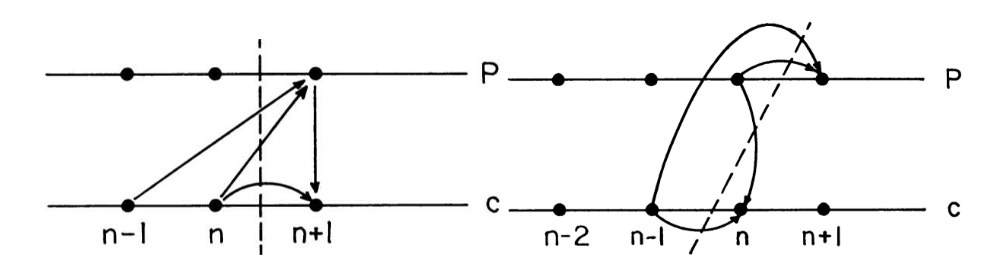
\includegraphics[width=\textwidth]{Miranker-Liniger.png}
    \end{frame}

    \begin{frame}
        \frametitle{Example: Miranker and Liniger (1967)}
        Predictor corrector method
        \[\begin{aligned}
            y^p_{n+1} &= y^c_n + 2hf(t, y^c_n)\\
            y^c_{n+1} &= y_n^c + \frac{h}{2}(f(t, y^p_{n}) + f(t, y^c_{n-1}))
        \end{aligned}\]
    \end{frame}

    \section{Parareal}
    \begin{frame}
        \frametitle{Parareal}
        \begin{itemize}
            \item Large scale method
            \item Iterative
            \item Easy to implement
            \item Coarse (and cheap!) method $y_{i+1} = \mathcal{G}(y_i, t_i, t_{i+1})$
            \item Fine method $y_{i+1} = \mathcal{F}(y_i, t_i, t_{i+1})$
        \end{itemize}
    \end{frame}

    \begin{frame}
        \frametitle{Parareal}
        \[y_{j+1}^{k+1} = \mathcal{G}(y^{k+1}_j, t_j, t_{j+1}) + \mathcal{F}(y^k_j, t_j, t_{j+1}) - \mathcal{G}(y^k_j, t_j, t_{j+1})\]
    \end{frame}

    \begin{frame}
        \frametitle{Example: damped harmonic oscillator}
        \[y'' + 2\zeta \omega_0 y' + \omega_0^2 y = 0\]\vspace{20pt}
        \[\begin{aligned}
            q' &= p\\
            p' &= -2\zeta \omega_0 p - \omega_0^2 q
        \end{aligned}\]
    \end{frame}
    \begin{frame}
        \begin{center}
        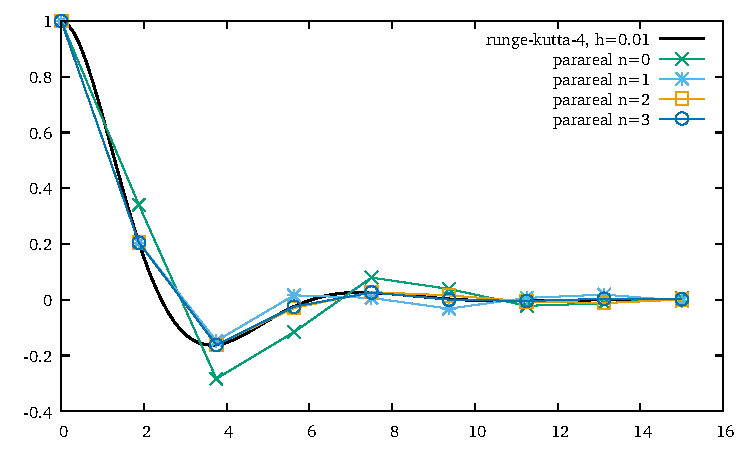
\includegraphics[width=0.8\textwidth]{plot1.pdf}
        \end{center}
    \end{frame}

    \begin{frame}
        \frametitle{Instability}
        For most (interesting) problems (hyperbolic equations, Navier-Stokes with large Reynolds number) 
        \begin{itemize}
            \item Convergence is too slow
        \end{itemize}
        or
        \begin{itemize}
            \item Parareal is unstable
        \end{itemize}
        Modifications and enhancements exist.
    \end{frame}

    \section{MultiGrid}
    \begin{frame}
        \begin{itemize}
            \item Generalisation of Parareal
            \item Extend (spatial) MultiGrid method to time domain
            \item Non-intrusive
            \item Implemented in C++ $\to$ XBraid
        \end{itemize}
    \end{frame}

    \section{PFASST}
    \begin{frame}
        \begin{itemize}
            \item Parallel Full Approximation Scheme in Space-Time
            \item deferred correction method (See Gander 50 years paper)
            \item Shows promise in practice, but convergence behaviour is not fully understood.
            \item Implemented in C++ $\to$ PFASST++
        \end{itemize}
    \end{frame}

    \section{Conclusion}
    \begin{frame}
        \begin{itemize}
            \item Active community: parallel-in-time.org (software directory)
        \end{itemize}
    \end{frame}
\end{document}
